\documentclass[a4paper,amsmath]{oblivoir}

\usepackage{fapapersize}
\usefapapersize{*,*,1in,*,1in,*}

\makeatletter
\let\ATonum\@onum
\makeatother

\usepackage{esgutil}
\usepackage{refcount}


\usepackage{xcolor}
\usepackage{graphicx}
\usepackage{hologo}
\usepackage{relsize}
\usepackage{tcolorbox}
\tcbuselibrary{listings,breakable}
\tcbset{listing engine=listings,colframe=cyan,colback=cyan!5!white}

\setmainfont{TeX Gyre Pagella}
\setsansfont{Noto Sans}
\setmonofont{Noto Sans Mono}
\setkomainfont(Noto Serif CJK KR)(* Bold)(Noto Sans CJK KR)
\setkosansfont[Noto Sans CJK KR]()( Bold)( Medium)
\usepackage{unicode-math}
\setmathfont{texgyrepagella-math.otf}

\newcounter{sub}
\newcommand\bangotsuite{\stepcounter{sub}\thesub}

\usepackage{tikz}
\newcommand\tikzlogo{Ti\textit{k}Z}

\setlength{\parindent}{0mm}

\newcommand\pkg[1]{\textsf{#1}}

\ExplSyntaxOn 

\NewDocumentEnvironment {intro} {o}
{
    \IfValueTF { #1 }
    {
        \int_set:Nn \l_tmpa_int { #1 }
    }
    {
        \int_set:Nn \l_tmpa_int { 1 }
    }
    \noindent \rule {\linewidth}{3pt}
    \par 
    \sffamily [No.\space\int_use:N \l_tmpa_int ]\ \ 
    \bfseries
}
{
    \hfill \underline{\hphantom{2019}}년~\underline{\hphantom{06}}월~ \underline{\hphantom{25}}일 
    \par 
    \vskip -.3\baselineskip 
    \noindent \rule {\linewidth }{1pt}
    \par 
    \vskip .5\baselineskip 
}

\NewDocumentCommand \exverb { d|| }
{
    \texttt { \tl_to_str:n { #1 } }
}

\ExplSyntaxOff 

\NewDocumentEnvironment {questiona} { m }
{
%    \medskip
    \begin{tcolorbox}[title={#1},fonttitle={\sffamily\bfseries}]
}{%
    \end{tcolorbox}
}

\NewDocumentEnvironment {questionp} { }
{
%    \medskip
    \begin{tcolorbox}[colframe=orange!30!black!60,colbacktitle=orange!25!gray,
    title={연습문제},fonttitle={\sffamily\bfseries}]
}{%
    \end{tcolorbox}
}


\NewDocumentEnvironment {exampleonly} {}
{%
%    \begin{tcblisting}{listing only}
    \expandafter\tcblisting{listing only,breakable,before={\par\medskip\setstretch{1}}}
}{
    \endtcblisting
%    \end{tcblisting}
}

\NewDocumentEnvironment {exampleside} {}
{%
    \tcblisting{listing side text,righthand width=.35\textwidth,breakable,before={\par\medskip\setstretch{1}}}%
}{%
    \endtcblisting
}

%\NewDocumentEnvironment {examplebelow} {}
%{%
%    \medskip
%    \tcblisting{text below listing,breakable}%
%}{%
%    \endtcblisting
%}
\newtcblisting{examplebelow}{breakable,before={\par\medskip\setstretch{1}}}

\begin{document}

\begin{intro}[5]
Dim and Dimmer
\end{intro}

\begin{questiona}{문제}
현재 조판하고 있는 페이지의 메트릭을 mm 단위로 보여주는 명령 \verb|\currentmetric|을 작성하여라.
\tcblower
입력: \verb|\currentmetric{textwidth}| \\
출력: 184.4mm
\end{questiona}

\section{\TeX 의 dimension과 expl3의 \textsf{dim} 데이터타입}

\paragraph{\TeX 의 길이 단위 연산자}

\TeX 은 내부적으로 모든 길이를 sp로 계산한다. 사용자 인터페이스에서는 pt를 기본 단위로 쓴다. 1pt $ = $ 65536sp이다. 다음은 미리 정의된 길이 단위 연산자들이다.
\begin{quote}
sp, pt, mm, cm, in \\
bp, pc, dd, cc, nd, nc
\end{quote}
폰트에 따라 가변적 값을 가지는 두 가지 단위가 있다.
\begin{quote}
em, ex
\end{quote}

\TeX 에서 사용하는 point는 소위 “작은 포인트”로서 $1/72.27$인치에 해당한다. 반면 PostScript 포인트를 “큰 포인트”라고 하고 이것은 $1/72$인치이다. 이에 해당하는 단위는 bp이다.

em과 ex는 폰트의 \dotemph{디자인}에 관련되는 단위이다. em은 “대문자 M의 width”라는 의미에서 나온 말이지만 현대의 많은 폰트에서 대문자 M은 실제로 1em을 넘거나 모자라는 경우가 많다. 이것은 전적으로 디자인 문제라고 생각하면 된다. 글자를 디자인하는 정사각형 디자인 박스의 가로세로 폭을 1em이라고 하는데, 이를 1000으로 설정한 다음 이 정사각형 안에 글자 모양을 그려넣는 것이 일반적이다. 현재 이 문서의 영문자는 TeX Gyre Pagella를 쓰고 있는데 M자의 폭과 1em의 길이를 구해보면
\begin{exampleside}
\ExplSyntaxOn
\hbox_set:Nn \l_tmpa_box { M }
\dim_eval:n { \box_wd:N \l_tmpa_box } \\
\dim_eval:n { 1em }
\ExplSyntaxOff
\end{exampleside}
즉, 폰트 사이즈가 10pt일 때 1em은 10pt이지만 M자의 width는 디자인에 따라 달라진다.

한편 ex는 x자의 높이라는 의미인데, 이 역시 디자인 상의 단위이다. 라틴 문자는 4개의 선을 그어놓고 알파벳을 디자인한다고 생각할 때, 아래에서 두 번째 줄이 베이스라인이고 베이스라엔에서 그 다음 세 번째 줄까지의 길이를 ex라고 하는 것이다. em과 달리 이 길이는 폰트마다 다 다르고 폰트 사이즈에 따라서도 달라진다. 실제 식자되는 x자의 높이와 거의 같다.

\begin{exampleside}
\ExplSyntaxOn
\hbox_set:Nn \l_tmpa_box { x }
\dim_eval:n { \box_ht:N \l_tmpa_box } \\
\dim_eval:n { 1ex }
\ExplSyntaxOff
\end{exampleside}


\paragraph{dim 데이터타입}

\verb|\dim_eval:n|의 인자로 dim 표현식이 오는 것은 다른 “수”의 경우와 똑같다. 내부적으로 dim은 fp와 비슷한 모양을 하고 있지만 그것은 우리가 interface 단위로서 pt를 채택하고 있어서 그럴 뿐이고 실제로는 sp 단위의 정수 연산을 하고 있다.

dim 변수는 길이를 요구하는 모든 곳에 적용가능하다.

dimension 표현식은 반드시 단위 연산자가 붙는다. 예를 들면
\begin{exampleonly}
\dim_set:Nn \l_tmpa_dim { 29.92 }
\end{exampleonly}
이것은 단위가 붙지 않았다는 오류를 낸다. 그렇다면 fp 표현식에 단위 연산자를 붙이면 dim에 할당이 될까?

\begin{exampleside}
\ExplSyntaxOn
\dim_set:Nn \l_tmpa_dim { \fp_eval:n { 19.6 / 2.7 } pt }
\rule{\l_tmpa_dim}{5pt}
\ExplSyntaxOff
\end{exampleside}

일반적으로 말해서 fp보다는 dim 계산이 빠르다. 그러므로 위와 같은 것은 가능은 한데 dim으로 계산할 수 있다면 그것이 더 좋다.

dim 표현식은 fp만큼 유연하지 않다. 예를 들면 
\begin{exampleside}
\ExplSyntaxOn
\dim_set:Nn \l_tmpa_dim { 10pt }
\dim_eval:n { 2\l_tmpa_dim + 4pt } \\
\dim_eval:n { \l_tmpa_dim * 2 + 4pt }
\ExplSyntaxOff
\end{exampleside}
이와 같이 “계수에 의한 곱연산”이 가능하지만
\begin{exampleonly}
\ExplSyntaxOn
\dim_eval:n { 0.333*2*\l_tmpa_dim + 2pt }
\ExplSyntaxOff
\end{exampleonly}
곱셈을 연산처럼 중첩해서 쓰지 못한다.

나눗셈은 다음과 같이 쓴다. \verb|\dim_ratio:nn| 함수는 인자 두 개를 다 dim으로만 받아들여서 fp 결과를 되돌리기 때문에 단위에 주의하여야 한다.
\begin{exampleside}
\ExplSyntaxOn
\dim_eval:n { 10pt / 2 } \\
\dim_eval:n { 10pt * \dim_ratio:nn {10pt} {2pt} }
\ExplSyntaxOff
\end{exampleside}

dim 표현식은 확장 순서에 매우 민감하다. 예를 들면
\begin{verbatim}
\dim_eval:n { 10pt * \dim_ratio:nn {10pt} {2pt} }
\end{verbatim}
이것은 오류를 일으키지 않지만
\begin{verbatim}
\dim_eval:n { \dim_ratio:nn {10pt} {2pt} * 10pt }
\end{verbatim}
이것은 evaluate에 실패하였다는 메시지를 볼 수 있다. 그 이유는 
\begin{verbatim}
\dim_eval:n { 2 * 20pt }
\end{verbatim}
이것은 실패이지만
\begin{exampleside}
\ExplSyntaxOn
\dim_eval:n { 20pt * 2 }
\ExplSyntaxOff
\end{exampleside}
이것은 성공하는 것과 정확하게 같다.

\paragraph{길이를 fp로 계산하기}

그래서 가끔 아주 복잡한 길이 계산을 해야 할 때는 단위를 다 떼어놓고 fp로 계산한 다음 그 결과에 단위를 다시 붙여주는 것이 (코딩하기) 편할 때가 있다.


아주 오랜 옛날부터 \verb|\strip@pt|라는 트릭이 있었다.
\begin{examplebelow}
\makeatletter
\strip@pt\textwidth
\makeatother
\end{examplebelow}
이렇게 해놓고 이것을 fp처럼 계산하겠다는 것이지. 이를 이용하여 다음 문제를 풀어보자.

\begin{questiona}{보충문제}
현재 폰트 현재 폰트사이즈에서 알파벳 대문자 M의 폭/높이(width/height)의 값을 나타내어라.
\end{questiona}

expl3를 모를 때 어떻게 했는지 기억을 되살려보면,

\begin{examplebelow}
\newsavebox\M \sbox\M{M}
\newdimen\Mwidth\newdimen\Mheight
\Mwidth=\wd\M \Mheight=\ht\M
\the\Mwidth, \the\Mheight \\
\makeatletter
\strip@pt\Mwidth, \strip@pt\Mheight
\makeatother
\end{examplebelow}
이제 실수 나눗셈을 하면 되는데 이것은 fp나 realcalc 또는 calc 패키지를 이용하여 할 수 있을 듯하다.

expl3로는 아마 이렇게 할 수 있지 않을까?
\begin{examplebelow}
\ExplSyntaxOn
\hbox_set:Nn \l_tmpa_box { M }
\dim_set:Nn \l_tmpa_dim { \box_wd:N \l_tmpa_box }
\dim_set:Nn \l_tmpb_dim { \box_ht:N \l_tmpa_box }
\fp_eval:n { \dim_ratio:nn { \l_tmpa_dim } { \l_tmpb_dim } }
\ExplSyntaxOff
\end{examplebelow}

\paragraph{참고, hbox와 dimension}

아까부터 \verb|\hbox_...| 어쩌고 하는 명령이 나오는데 
\textsf{box} 데이터타입에 대하여 따로 상세히 배우게 된다.

지금은 다음과 같은 것을 능숙하게 할 수 있도록 해두자.

다른 타입과 마찬가지로 네 개의 scratch 변수가 주어져 있다.
지금은 vbox에 대하여 신경쓸 것 없이 hbox만을 알아두면 된다.
hbox란 horizontal mode의 box라는 뜻이다.

여기에 식자할 material을 집어 넣는 것은
\begin{exampleonly}
\hbox_set:Nn \l_tmpa_box { material }
\end{exampleonly}

이것을 typeset 하려면
\begin{exampleonly}
\box_use:N \l_tmpa_box
\end{exampleonly}

주어진 box의 폭(width), 높이(height), 깊이(depth)는 다음과 같이 측정하는데 그 결과는 dim이다.
\begin{exampleonly}
\box_wd:N \l_tmpa_box
\box_ht:N \l_tmpa_box
\box_dp:N \l_tmpa_box
\end{exampleonly}


\includegraphics[scale=2]{dimofbox}

totalheight는 ht+dp를 말한다.
\begin{examplebelow}
\ExplSyntaxOn
\hbox_set:Nn \l_tmpa_box { Study~Group }
width:~\dim_eval:n { \box_wd:N \l_tmpa_box } \\
height:~\dim_eval:n { \box_ht:N \l_tmpa_box } \\
depth:~\dim_eval:n { \box_dp:N \l_tmpa_box } \\
totalheight:~
\dim_set:Nn \l_tmpa_dim { \box_ht:N \l_tmpa_box + \box_dp:N \l_tmpa_box }
\dim_use:N \l_tmpa_dim
\ExplSyntaxOff
\end{examplebelow}

\paragraph{지금 이 긴 이야기의 결론은} 사용자 레벨에서 “단위가 제거된 dim은 fp”라는 것이다. 그렇다면 dim의 단위를 제거하려면 어떻게 하는가?

\verb|\dim_to_decimal:n|은 모든 길이를 pt로 환산한 다음 단위를 제거해준다. 이것은 \verb|\strip@pt|의 expl3 판이라고 해도 좋겠다. 단 이 명령은 소수 다섯째 자리까지 유효한 근삿값이다.

\begin{examplebelow}
\ExplSyntaxOn
\dim_to_decimal:n { \textwidth }
\ExplSyntaxOff
\end{examplebelow}

현재 페이지의 종횡비(세로/가로)를 구해보자.
\begin{examplebelow}
\ExplSyntaxOn
\fp_eval:n 
  {
     \dim_to_decimal:n { \paperheight } 
     / 
     \dim_to_decimal:n { \paperwidth } 
  }
\ExplSyntaxOff
\end{examplebelow}

A4 페이퍼는 접어도 종횡비가 유지되는 판형이다. 즉 세로 길이가 가로 길이의 $\sqrt{2}$배이다.

\paragraph{단위 간의 변환}

\verb|\dim_to_decimal_in_unit:nn| 함수가 제일 요긴하다. 두 번째 인자에 표시하고 싶은 단위를 써주면 된다. 10포인트가 몇 mm인지를 나타내려면
\begin{exampleside}
\ExplSyntaxOn
\dim_to_decimal_in_unit:nn { 10pt } { 1mm }
\ExplSyntaxOff
\end{exampleside}
이 함수 연산의 결과는 dim 형이 아니라는 점을 기억해야 한다. 단위가 따로 붙어 있지 않다. 
그러므로 fp에 할당하여 연산할 수 있으며 tl에 할당하는 것도 가능하다.
표현 시에는 mm를 적어주어야 한다.

\paragraph{dim 조건식}

\verb|\int_compare:nTF|와 마찬가지로 \verb|\dim_compare:nTF|가 있다. 
\begin{examplebelow}
\ExplSyntaxOn
\dim_set_eq:NN \l_tmpa_dim \textwidth
\dim_set_eq:NN \l_tmpb_dim \linewidth

\dim_compare:nTF { \l_tmpa_dim - \l_tmpb_dim == \c_zero_dim }
{
    textwidth == linewidth
}
{
    textwidth != linewidth
}
\ExplSyntaxOff
\end{examplebelow}
길이를 비교하는 것은 문제가 없지만 위의 경우처럼 0보다 큰가 작은가를 비교할 때 자주 하는 실수가 
\begin{verbatim}
\dim_compare:nTF { \l_tmpa_dim == 0 }
\end{verbatim}
과 같이 그냥 0와 비교하려 하는 것이다. 이것은 실패.
반드시 0pt와 비교하여야 한다. 이것이 실수하기 쉬우므로 
\begin{exampleonly}
\c_zero_dim
\end{exampleonly}
이라는 상수를 쓰는 것이 좋다. 이것은 그냥 0pt이다.

이밖에 while do와 같은 반복문도 있으므로 int가 아니라 길이가 문제일 때는 dim 자료형을 쓴다고 생각하여도 무방하다.


\bigskip

이제 주어진 문제를 해결해보자. 인자로 들어오는 길이 변수 이름이 만약 존재하지 않는 것이면 이를 에러처리하는 것을 포함한다. 

소수 다섯째 자리가 너무 길고 눈에 들어오지 않으니까 최대 소수 둘째 자리까지만 보여주기로 하자.

\begin{examplebelow}
\ExplSyntaxOn
\NewDocumentCommand \currentmetric { m }
{
    \dim_if_exist:cTF { #1 }
    {
        \calc_metric_fn:n { #1 }
    }
    {
        \texttt{\bs #1}~is~invalid
    }
}

\cs_new:Npn \calc_metric_fn:n #1
{
    \dim_set_eq:Nc \l_tmpa_dim { #1 }
    
    \texttt{\bs #1} $\,=\,$
    
    \fp_eval:n { round ( \dim_to_decimal_in_unit:nn { \l_tmpa_dim } { 1mm } , 2 ) }
    \,mm
}

\ExplSyntaxOff

\currentmetric{hello}

\ExplSyntaxOn
\dim_new:N \hello \dim_set:Nn \hello { .33\textwidth }
\ExplSyntaxOff

\currentmetric{hello}

\currentmetric{foremargin}
\end{examplebelow}

간단하지만 의외로 요긴한 명령이다. \textsf{printlen}이라는 패키지가 길이 단위를 제어할 수 있게 해주는데 생각해보면 패키지까지 써야 하는지 의문이기는 하다.

\vfill

%\ExplSyntaxOn
%\fp_eval:n { \dim_to_decimal_in_unit:nn { 1pt } { 1mm } }
%\fp_eval:n { \dim_to_decimal_in_unit:nn { 1mm } { 1pt } }
%\ExplSyntaxOff


\begin{questionp}
\fbox{기본} 1. 다음 도표의 빈 칸을 채워 완성하여라.
\begin{tabular}{c|c|c|c|c}
   & pt & mm & pc & in \\ \hline
pt &  1.00000  & 0.35146  &	  &  \\ \hline
mm & 2.84526  & 1.00000   &	  &  \\  \hline
pc &    &    & 1.00000	  &  \\ \hline
in &    &    &	  & 1.00000 \\ \hline
\end{tabular}

\bigskip

\fbox{기본} 2. \LaTeX 에 \verb|\settowidth|와 \verb|\settoheight|, \verb|\settodepth|라는 명령이 있다. 이의 사용법은 다음과 같다.

\begin{exampleside}
\newlength{\mylen}
\settowidth{\mylen}{beautiful}
\the\mylen
\end{exampleside}

이것과 동일한 작용을 하는 \verb|\SettoWidth|, \verb|\SettoHeight|, \verb|\SettoDepth|를 expl3로 만들고 \verb|\SettoTotalheight|도 작성해보아라. 

\bigskip

\fbox{기본} 3. 다음 문장에서, 각 단어의 (문장부호를 제외한) 길이를 측정하여 평균값을 구하고, 그 문단의 margin에 \verb|\rule{<평균값>}{10pt}|의 막대를 그려라.

\begin{framed}
남방의 비는 차갑고 단단하고 찬란한 눈꽃으로 변하는 일이 절대 없다. 식자들은 남방의 비가 단조롭다고 생각하는데 비 자신도 그것을 불행으로 여기는지 어떤지, 강남의 눈은 그래도 촉촉하고 윤기가 돌아 아름답기 그지없다. 그것은 아직 눈뜨지 않은 청춘의 소식이며, 건강한 처녀의 살결이다. 

눈 덮인 들에는 핏빛의 붉은 동백이며, 흰빛에 푸르름이 감도는 외겹 매화며, 경쇠 모양의 진노랑 새양꽃이 있고, 눈 밑에는 아직도 파랗게 언 잡초들이 있다. 나비는 분명 없었다. 꿀벌이 동백꽃과 매화꽃의 꿀을 따러 왔었는지 아닌지, 나는 확실히 기억할 수 없다. 단지 나의 눈앞에는 겨울꽃이 핀 눈 덮인 들판에 바쁘게 날아다니는 수많은 벌들이 보이는 듯, 시끄럽게 붕붕거리는 소리가 들리는 듯했다.
\end{framed}



\bigskip

\fbox{기본} 4. 다음 표를 완성하고 1em의 크기가 fontsize에 따라 어떻게 달라지는지 조사하여라. 만약 문서 폰트 크기 옵션이 10pt가 아니라 11pt 또는 12pt가 되면 이 값이 어떻게 변하는지도 조사하여라.

\begin{center}
\ExplSyntaxOn

\begin{tabular}{r|r}
\hline
font~size~command & value~of~em \\ \hline
\bs scriptsize & \scriptsize \dim_eval:n { 1em } \\ \hline
... & ... \\ \hline
\bs large & \large \dim_eval:n { 1em } \\ \hline
... & ... \\ \hline
\end{tabular}
\ExplSyntaxOff
\end{center}

\end{questionp}

%
%
%\makeatletter
%\newlength\LC@temph\newlength\LC@tempw\newlength\LC@tempwtwo
%\newlength\LC@templ
%\newcommand*{\lccompthreevar}[5]{%
%\settowidth{\LC@temph}{$\scriptstyle #2$}
%\settowidth{\LC@tempw}{$\scriptstyle #3$}
%\settowidth{\LC@tempwtwo}{$\scriptstyle #3$}
%\settowidth{\LC@templ}{$\scriptstyle #4 #5$}
%{#1}{}_{\substack{#2 #3 #4 #5\\\makebox[\LC@temph]{\hfill$\scriptstyle 1$\hfill}%
%\makebox[\LC@tempw]{\hfill\phantom{$\scriptstyle 2$}\hfill}%
%\hspace{\LC@templ}%
%}}^{\hspace{\LC@temph}\hspace{\LC@tempw}\makebox[\LC@tempwtwo]{\hfill$\scriptstyle 3$\hfill}}
%}
%\makeatother
%
%\begin{questionp}
%\fbox{실력} 5. 다음과 같은 식을 만들어야 한다고 하자.
%\[
%{}_n\lccompthreevar{Q}{x}{y}{z}{}
%\]
%이와 같은 식을 식자하는 \verb|\mycmd{Q}{n}{x}{y}{z}{1}{3}|와 같은 명령을 작성하되,
%각 인자의 의미가 다음과 같도록 하여라.
%\begin{enumerate}[\expandafter\ATonum1] \tightlist
%\item \verb|#2|는 \verb|#1|의 왼쪽에 오는 하첨자이다.
%\item \verb|#3, #4, #5| 세 개는 \verb|#1|의 오른쪽에 오는 하첨자이다.
%\item \verb|#6|에는 한 자리 숫자가 오는데 그 값은 3이하이다. 이 숫자에 따라 x, y, z의 해당 위치 아래(예컨대 1이면 x의 아래, 2이면 y의 아래)에 scriptsize로 식자한다.
%\item \verb|#7|은 \verb|#6|과 같이 하되, 하첨자의 위쪽에 식자한다.
%\end{enumerate}
%
%\end{questionp}


\newpage

\begin{questiona}{문제}
인자로 주어지는 각 글자를 \verb|\colorbox|에 넣어라. 배경색상을 임의로 설정하고 전경색상은 그 반전색으로 하라. 띄어쓰기는 무시한다. 칼라 모델은 \textsf{xcolor}의 rgb나 HTML을 사용하여라. 
\tcblower
입력: \verb|\mytest{우리나라}|\\
출력: \definecolor{ba}{rgb}{.1,.2,.3}%
\definecolor{fo}{rgb}{.9,.8,.7}%
\colorbox{ba}{\color{fo}우}%
\definecolor{ba}{rgb}{.3,.6,.8}\definecolor{fo}{rgb}{.7,.4,.2}%
\colorbox{ba}{\color{fo}리}%
\definecolor{ba}{rgb}{.5,.2,.8}\definecolor{fo}{rgb}{.5,.8,.2}%
\colorbox{ba}{\color{fo}나}%
\definecolor{ba}{rgb}{.6,.2,.1}\definecolor{fo}{rgb}{.4,.8,.1}%
\colorbox{ba}{\color{fo}라}%
\end{questiona}

\section{\protect\TeX 의 가상난수}

원래 \TeX 에는 난수생성기가 없었다. \TeX{} 엔진 자체에서 난수를 생성할 수 있게 된 것은 
pdf\TeX 이 처음이었다.
그 이전에는 \textsf{random.tex}이라는 작은 유틸리티, \textsf{lcg} 패키지 등이 난수를 흉내내었고,
\textsf{pgf} 계산 엔진이 개발된 후에는 \textsf{pgfmath}에서 난수를 생성해주게 되었다.

expl3의 난수 엔진은 \textsf{pgfmath}의 것을 쓰지 아니하고 엔진 자체의 primitive를 활용한다.
pdf\TeX 에는 
\begin{verbatim}
\pdfnormaldeviate
\pdfuniformdeviate
\end{verbatim}
라는 두 개의 primitive가 있으며 \hologo{LuaTeX}과 \hologo{XeTeX}에는 
\begin{verbatim}
\normaldeviate
\uniformdeviate
\end{verbatim}
가 마련되어 있다. 특히, \hologo{XeTeX}의 난수 프리미티브는 2019년 버전에서 처음으로 도입된 것이다.
\TeX\,Live 2018까지는 이 기능을 \hologo{XeTeX}에서 사용할 수 없다.

정규분포 난수 생성 명령인 normaldeviate에 대해서는 나중에 기회가 닿으면 살펴보기로 하고 우리는 uniform deviate에 대해서만 다루겠다.

따로 seed를 정해주지 않으면 (다른 언어들이 그리 하듯이) 시스템 시간을 seed로 하여 가상 난수를 생성한다.
(seed를 설정하거나 재설정하는 것이 가능하지만 이 문제는 당분간 논외로 한다.)

프리미티브를 직접 사용하는 예를 들어보겠다.

\begin{exampleside}
\ifPDFTeX
    \let\uniformdeviate\pdfuniformdeviate
\fi
\uniformdeviate 100 
\end{exampleside}
\verb|\uniformdeviate n|이 생성하는 난수는 $0 \le x < n$ 범위의 정수이다.
이 프리미티브들은 \emph{The Art of Computer Programming}의 제2권 3장 6절에 나오는 내용을 \hologo{METAPOST}로 구현한 것이다.
expl3는 전적으로 각 엔진의 프리미티브에 의존한다.

정수형 난수를 얻는 함수는 다음과 같다.
\begin{exampleside}
\ExplSyntaxOn
\int_rand:n { 100 } \\
\int_rand:nn { 10 } { 20 }
\ExplSyntaxOff
\end{exampleside}

앞서 본 프리미티브 자체와는 달리 expl3 함수는 주어진 수를 포함한다. 인자가 두 개인 함수가 만드는 난수의 범위는 $n_1 \le x \le n_2$이다. \verb|\int_rand:n {a}|는 \verb|\int_rand:nn {1}{a}|와 같다.


0이상 1미만의 실수형 난수를 얻는 방법은 다음과 같다.
\begin{exampleside}
\ExplSyntaxOn
\fp_eval:n { rand () }
\ExplSyntaxOff
\end{exampleside}
해상도는 fp 자체의 significand와 동일하게 $10^{-16}$이다. fp 자료형에도 정수형 난수를 얻는 randint가 있지만 정수 계산은 \verb|\int_rand:|가 더 빠르고 좋다.
주의할 것은 fp의 rand() 함수는 위쪽 경계 1을 포함하지 않는다는 점이다.

\bigskip

주어진 문제를 해결하기 위해 세 개의 int 변수를 만들고 이 각각에 random으로 100 이하의 정수값을 주기로 한다.
이 값을 100으로 나누어서 R, G, B의 각 색상값으로 삼아보겠다. fp random을 쓰지 않고 int random을 쓰는 이유는 무엇보다 그것이 빠르기 때문이고 색상 표현을 위해 R, G, B 각각 100분할 정도면 충분하다고 생각하기 때문이다.

\begin{examplebelow}
\ExplSyntaxOn
\int_new:N \l_r_int
\int_new:N \l_g_int
\int_new:N \l_b_int
\tl_new:N \l_r_tl
\tl_new:N \l_g_tl
\tl_new:N \l_b_tl

\cs_new:Nn \gen_rand_color:
{
    \int_set:Nn \l_r_int { \int_rand:nn { 0 } { 100 } }
    \int_set:Nn \l_g_int { \int_rand:nn { 0 } { 100 } }
    \int_set:Nn \l_b_int { \int_rand:nn { 0 } { 100 } }
    \tl_set:Nf \l_r_tl { \fp_eval:n { \l_r_int / 100 } }
    \tl_set:Nf \l_g_tl { \fp_eval:n { \l_g_int / 100 } }
    \tl_set:Nf \l_b_tl { \fp_eval:n { \l_b_int / 100 } }
    
    \exp_args:Nnnx \definecolor{back}{rgb}{\l_r_tl,\l_g_tl,\l_b_tl}
    
    \int_set:Nn \l_r_int { 100 - \l_r_int }
    \int_set:Nn \l_g_int { 100 - \l_g_int }
    \int_set:Nn \l_b_int { 100 - \l_b_int }
    \tl_set:Nf \l_r_tl { \fp_eval:n { \l_r_int / 100 } }
    \tl_set:Nf \l_g_tl { \fp_eval:n { \l_g_int / 100 } }
    \tl_set:Nf \l_b_tl { \fp_eval:n { \l_b_int / 100 } }

    \exp_args:Nnnx \definecolor{fore}{rgb}{\l_r_tl,\l_g_tl,\l_b_tl}    
}

\gen_rand_color:
back:~{\color{back}\rule{20pt}{10pt}}\\
fore:~{\color{fore}\rule{20pt}{10pt}}

\ExplSyntaxOff
\end{examplebelow}

반복해서 같은 유형의 문장을 계속 쓰는 것이 싫은 사람도 있을 것이다.

\begin{exampleonly}
    \tl_set:Nf \l_r_tl { \fp_eval:n { \l_r_int / 100 } }
    \tl_set:Nf \l_g_tl { \fp_eval:n { \l_g_int / 100 } }
    \tl_set:Nf \l_b_tl { \fp_eval:n { \l_b_int / 100 } }
\end{exampleonly}

이것을 
\begin{exampleonly}
    \clist_set:Nn \l_cm_clist { r, g, b }
    \int_step_inline:nn { \clist_count:N \l_cm_clist }
    {
        \tl_set:cf { l_ \clist_item:Nn \l_cm_clist { ##1 } _ tl }
          { \fp_eval:n { \int_use:c { l_ \clist_item:Nn \l_cm_clist { ##1 } _ int } / 100 } }
    }
\end{exampleonly}
이렇게 쓸 수 있다는 것을 지적해둔다. 항목이 여러 개면 더 나은 방법이 될 때도 있다.

\bigskip

한 글자를 다음과 같이 찍을 수 있으므로 
\begin{examplebelow}
\ExplSyntaxOn

\cs_new:Npn \print_char:n #1
{
    \gen_rand_color:
    \colorbox{back}{\color{fore} #1}
}

\print_char:n {H}

\ExplSyntaxOff
\end{examplebelow}

원하는 명령을 작성할 수 있게 되었다.

\begin{examplebelow}
\ExplSyntaxOn
\NewDocumentCommand \colorful { m }
{
    \tl_map_inline:nn { #1 }
    {
        \print_char:n { ##1 }
    }
}

\ExplSyntaxOff

\colorful{Hello}
\end{examplebelow}

컴파일할 때마다 색상 배열이 달라질 것이다. 알록달록 예쁘기만 하면 된다.

여기서는 전경색과 배경색을 단순히 100에서 뺀 R, G, B 값을 가지고 만들었지만
실제로는 색상에 대한 이해와 토론이 필요한 주제이다. 이에 대하여 더 다루지 않는다.

\vfill

\begin{questionp}
\fbox{기본} 1. 심심해진 철수는 idle 프로그램으로 다음과 같은 것을 하면서 놀았다.

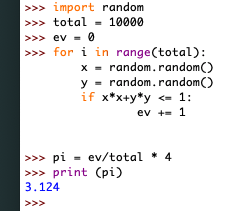
\includegraphics[scale=.9]{Screenshot-5-1}

이것을 본 영희가 “나는 expl3로 할 수 있어”라고 하였다. 과연 할 수 있었을까?

\bigskip

\fbox{기본} 2. 등거리 random walk을 모사하려고 한다. 회전각을 난수적으로 얻어서
20회 정도 진행한 궤적을 \tikzlogo 로 나타내어라. 진행 거리는 0.5cm이다.

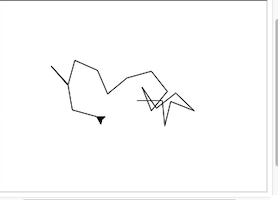
\includegraphics[scale=.9]{Screenshot-5-2}

\end{questionp}



\vfill
\hfill Nova de Hi.


\end{document}

